%Version 3 December 2023
% See section 11 of the User Manual for version history
%
%%%%%%%%%%%%%%%%%%%%%%%%%%%%%%%%%%%%%%%%%%%%%%%%%%%%%%%%%%%%%%%%%%%%%%
%%                                               
                  %%
%% Please do not use \input{...} to include other tex files.       %%
%% Submit your LaTeX manuscript as one .tex document.              %%
%%                                                                 %%
%% All additional figures and files should be attached             %%
%% separately and not embedded in the \TeX\ document itself.       %%
%%                                                                 %%
%%%%%%%%%%%%%%%%%%%%%%%%%%%%%%%%%%%%%%%%%%%%%%%%%%%%%%%%%%%%%%%%%%%%%

%%\documentclass[referee,sn-basic]{sn-jnl}% referee option is meant for double line spacing

%%=======================================================%%
%% to print line numbers in the margin use lineno option %%
%%=======================================================%%

%%\documentclass[lineno,sn-basic]{sn-jnl}% Basic Springer Nature Reference Style/Chemistry Reference Style

%%======================================================%%
%% to compile with pdflatex/xelatex use pdflatex option %%
%%======================================================%%

%%\documentclass[pdflatex,sn-basic]{sn-jnl}% Basic Springer Nature Reference Style/Chemistry Reference Style


%%Note: the following reference styles support Namedate and Numbered referencing. By default the style follows the most common style. To switch between the options you can add or remove “Numbered” in the optional parenthesis. 
%%The option is available for: sn-basic.bst, sn-vancouver.bst, sn-chicago.bst%  
 
%%\documentclass[pdflatex,sn-nature]{sn-jnl}% Style for submissions to Nature Portfolio journals
%%\documentclass[pdflatex,sn-basic]{sn-jnl}% Basic Springer Nature Reference Style/Chemistry Reference Style
\documentclass[pdflatex,sn-mathphys-num]{sn-jnl}% Math and Physical Sciences Numbered Reference Style 
%%\documentclass[pdflatex,sn-mathphys-ay]{sn-jnl}% Math and Physical Sciences Author Year Reference Style
%%\documentclass[pdflatex,sn-aps]{sn-jnl}% American Physical Society (APS) Reference Style
%%\documentclass[pdflatex,sn-vancouver,Numbered]{sn-jnl}% Vancouver Reference Style
%%\documentclass[pdflatex,sn-apa]{sn-jnl}% APA Reference Style 
%%\documentclass[pdflatex,sn-chicago]{sn-jnl}% Chicago-based Humanities Reference Style

%%%% Standard Packages
%%<additional latex packages if required can be included here>

\usepackage{graphicx}%
\usepackage{multirow}%
\usepackage{amsmath,amssymb,amsfonts}%
\usepackage{amsthm}%
\usepackage{mathrsfs}%
\usepackage[title]{appendix}%
\usepackage{xcolor}%
\usepackage{textcomp}%
\usepackage{manyfoot}%
\usepackage{booktabs}%
\usepackage{algorithm}%
\usepackage{algorithmicx}%
\usepackage{algpseudocode}%
\usepackage{listings}%
\usepackage{float}%

%%%%

%%%%%=============================================================================%%%%
%%%%  Remarks: This template is provided to aid authors with the preparation
%%%%  of original research articles intended for submission to journals published 
%%%%  by Springer Nature. The guidance has been prepared in partnership with 
%%%%  production teams to conform to Springer Nature technical requirements. 
%%%%  Editorial and presentation requirements differ among journal portfolios and 
%%%%  research disciplines. You may find sections in this template are irrelevant 
%%%%  to your work and are empowered to omit any such section if allowed by the 
%%%%  journal you intend to submit to. The submission guidelines and policies 
%%%%  of the journal take precedence. A detailed User Manual is available in the 
%%%%  template package for technical guidance.
%%%%%=============================================================================%%%%

%% as per the requirement new theorem styles can be included as shown below
\theoremstyle{thmstyleone}%
\newtheorem{theorem}{Theorem}%  meant for continuous numbers
%%\newtheorem{theorem}{Theorem}[section]% meant for sectionwise numbers
%% optional argument [theorem] produces theorem numbering sequence instead of independent numbers for Proposition
\newtheorem{proposition}[theorem]{Proposition}% 
%%\newtheorem{proposition}{Proposition}% to get separate numbers for theorem and proposition etc.

\theoremstyle{thmstyletwo}%
\newtheorem{example}{Example}%
\newtheorem{remark}{Remark}%
\theoremstyle{thmstylethree}%
\newtheorem{definition}{Definition}%
\raggedbottom
%%\unnumbered% uncomment this for unnumbered level heads

\begin{document}

\title[Article Title]{Matrix-based imaging through dynamic scattering}
%Noninvasive microscopy through dynamic scattering

\author[1]{\fnm{Elad} \sur{Sunray}}
\equalcont{These authors contributed equally to this work.}

\author[1]{\fnm{Gil} \sur{Weinberg}}
\equalcont{These authors contributed equally to this work.}

\author[1]{\fnm{Benzy} \sur{Laufer}}
\equalcont{These authors contributed equally to this work.}

\author*[1]{\fnm{Ori} \sur{Katz}}\email{orik@mail.huji.ac.il}


\affil[1]{\orgdiv{Institute of Applied Physics}, \orgname{The Hebrew University of Jerusalem}, \orgaddress{\city{Jerusalem}, \postcode{9190401}, \country{Israel}}}


\maketitle
%PAPER MESSAGES:
% Matricial methods
% Complexity of reconstructions - SCI & Bispectrum (Supp)

%FIGURES:
% 1 - concept
% 2 - transmission diffuser
% 3 - transmission beads
% 4 - reflection fluorescence
% 5 - coherent diffuser - Benzy

\section*{Abstract} %230 words (LSA max 250 words)

Noninvasive optical-resolution imaging through and within complex scattering media presents a major challenge with implications across multiple fields. 
State-of-the-art techniques, such as reflection matrix methods and neural network approaches, rely on multiple measurements under different illuminations or detection, either controlled or random. However, these methods are challenging to implement in rapidly varying dynamic media due to the large number of measurements needed within the short timescales where the medium remains relatively unchanged.
Here, we show that due to the commutativity of convolution, dynamic scattering in isoplanatic imaging is mathematically analogous to dynamic illumination in static scattering media. This allows us to leverage the state-of-the-art matrix-based approaches that were developed for undoing scattering in static media, to rapidly varying dynamic scattering samples, enabling the reconstruction of complex widefield images from a small number of camera frames without requiring or assuming any correlations between consecutive frames. Specifically, we demonstrate that the covariance matrix of a set of camera frames of light scattered through a rapidly varying dynamic scattering sample has the same mathematical form as a reflection matrix of a static medium, with the hidden static target object playing the role of the scattering medium.
The generality of the concept enables us to image through dynamic scattering in several different imaging modalities and experimental settings, from incoherent fluorescence microscopy to coherence-gated holographic reflection imaging.
 
%Our approach offers an adaptable and robust solution for both coherent and incoherent imaging through rapidly varying media, a challenge prevalent across many fields, from remote sensing to biomedical imaging. Noninvasive optical-resolution imaging through and within complex scattering media presents a major challenge, with substantial implications across multiple fields. 
%While recent advancements in coherent and incoherent imaging through severe multiple scattering have been introduced by reflection-matrix processing, approaches that tackle dynamic scattering have been limited. 
%\textbf{* The state of the art of the field: reflection-matrix and neural-networks, both based on multiple measurements under dynamic modulated illumination or detection, which is challenging to perform in dynamic rapidly varying media.
%* here we show that due to commutativity property of convolution, dynamic scattering in isoplanatic imaging is mathematically analogous to dynamic illumination
%* show that  allows to apply state of the art matricial approaches on the covatiance matrix, reconstructing complex widefield images from a small number of camera frames/measurements, not requiring or assuming any corrrelations between consecutive frames.
%The generality of the concept allows us to demonstrate experimental imaging through dynamic scattering and aberrations in several imaging modalities: from incoherent fluorescence microscopy to coherence-gated holographic reflection imaging.}
%Here, we present a computational framework that extends existing reflection matrix-based imaging to dynamic scattering scenarios. 
%We show that one can replace dynamic illuminations in static media with randomly varying media and static illumination. 
%We experimentally demonstrate that a small number of measurements acquired under dynamic scattering conditions can effectively be used to construct a virtual reflection matrix. 
%Processing this matrix with an adapted scattering compensation algorithm allows the reconstruction of high-resolution images without spatial-light modulators or computationally intensive processing. 
%Our approach offers an adaptable and robust solution for both coherent and incoherent isoplanatic imaging through rapidly varying media, a challenge prevalent across many fields, from remote sensing to biomedical imaging. 
%This method opens new possibilities for advancements in various fields, including biomedical imaging and remote sensing, where dynamic scattering is a prevalent challenge. 


\section*{Introduction}

Optical imaging through scattering media poses a fundamental challenge and opportunity for optical imaging \cite{yoon2020deep,bertolotti2022imaging}, and is a field with intense active research and significant recent advancements. 
Imaging objects through rapidly changing environments, such as atmospheric turbulence \cite{mao2022single,cai2023convrt,zhang2024imaging}, biological tissues \cite{jang2015relation,horstmeyer2015guidestar}, or fog \cite{satat2018towards}, holds a unique importance in fields ranging from medical imaging, through remote sensing, to astronomical observations.

%The complexity of scattering phenomena has necessitated the development of sophisticated techniques to overcome the barriers to clear imaging.
Among the recently developed scattering-compensation techniques, reflection-matrix-based methods have emerged as essential tools for noninvasive computational imaging through such media. These approaches rely on dynamic (controlled \cite{kang17,badon2020distortion,zhang2023deep,lim2024multiphoton} or uncontrolled \cite{lee22,weinberg2023noninvasive,sunray2024beyond}) illumination of a static scene, allowing the measurement of the sample reflection matrix, and subsequent application of scattering compensation and image reconstruction algorithms. As a result of the relatively large number of required consecutive measurements, these techniques are inadequate to tackle rapidly varying scattering, such as those encountered in flowing blood, atmospheric turbulence, or fog.
%Recent advancements have extended these capabilities to random illumination, assuming a consistent stationary scatterer throughout the measurement period and randomly changing illuminations. 
%\textbf{Neural-networks}, Metzler - \textbf{slowly} varying scene.

Recently, approaches based on neural networks or online learning have been proposed to tackle dynamic aberrations or scattering computationally. Neural-networks-based approaches include supervised methods \cite{sun2019image,liu2024learning}, which heavily rely on training data and usually lack interpretability, and unsupervised methods using neural representations \cite{feng23,xie2024wavemo} 
%The\textbf{ lack of interpretability} in these methods makes it challenging to understand and trust their decision-making process, which is crucial in many applications, particularly in medical imaging.
that assumes slow, correlated temporal variations in the scattering medium, making it challenging to adapt to rapidly uncorrelated media. 
Online learning of the transmission matrix of dynamic media \cite{valzania2023online} has been demonstrated, but it too is limited to slowly temporally varying scattering. 
%Additionally, ultrasound modulation has been suggested \cite{ruan2020fluorescence}, although it necessitates a complex experimental setup, and is limited in imaging resolution to the acoustic focus size. %In the coherent domain, techniques such as time gating \cite{kanaev2018imaging} can be employed to image through media with a ballistic component, but these methods are incompatible with incoherent imaging.
Impressive efforts to computationally undo dynamic atmospheric turbulence by deep learning have been reported in recent years \cite{mao2022single,jiang2023nert,cai2023convrt,zhang2024imaging, zhang2024spatio}. However, these methods are specialized in low-order atmospheric aberrations and are not aimed at correcting complex scattering, such as that encountered in biological tissues or highly scattering layers.

% Alternatively, speckle correlation imaging techniques \cite{labeyrie1970attainment,katz14, edrei2016optical,salhov2018depth,wang2020imaging,rosenfeld2021acousto,wang2021non,zhang2023high,guo2023dynamic,zhu2024non} offer a pathway for single-shot image reconstruction through highly scattering media. These methods exploit the statistical properties of speckle patterns to recover image information. Despite this advantage, they are generally hindered by two notable drawbacks: their limited effectiveness under conditions of extreme scattering and their reliance on iterative phase retrieval, which lacks guaranteed convergence for complex targets. Overcoming the challenge of reconstruction convergence can be achieved through deterministic bispectrum reconstruction \cite{wu2016single,hwang2019fast,he2023recursion,han2024single}, leveraging the closure phase principle from radio-astronomy. However, this approach still demands capturing a large number of speckle grains and involves computationally intensive processing. These limitations underscore the necessity for more adaptable and robust imaging strategies.

% speckle-correlations / stellar-speckle interferometry
Alternatively, speckle-correlation imaging techniques, inspired by stellar speckle interferometry \cite{labeyrie1970attainment}, which exploit the statistical properties of speckle patterns to recover image information, have been applied to varying scattering conditions \cite{labeyrie1970attainment,rosenfeld2021acousto,wang2021non,zhang2023high,guo2023dynamic} and, under certain conditions, can function as single-shot imaging techniques \cite{bert12,katz14, edrei2016optical,salhov2018depth,wang2020imaging,zhu2024non,makowski2024low}. 
However, despite this advantage, these techniques are hindered by their limitation to reconstruct only simple objects and their reliance on iterative phase retrieval \cite{fienup1978reconstruction}, which lacks guaranteed convergence. 
%While overcoming the reconstruction convergence challenge of phase retrieval can be achieved by deterministic bispectrum reconstruction \cite{wu2016single,hwang2019fast,he2023recursion,han2024single}.
% leveraging the closure phase principle from radio astronomy.
%, this still demands averaging the speckle correlations from a large number of speckle grains and involves computationally intensive processing. These limitations underscore the necessity for more adaptable and robust imaging strategies.
While deterministic bispectrum reconstruction \cite{wu2016single, hwang2019fast, he2023recursion, han2024single} can address the convergence challenge of phase retrieval, it still requires averaging a large number of speckle grains, limiting the reconstruction to simple objects.
These limitations underscore the need for an imaging technique that is inherently adapted to image complex scenes through rapidly varying media.

Recently, approaches based on neural networks or online learning have been proposed to tackle dynamic aberrations or scattering computationally. Neural-networks-based approaches include supervised methods \cite{sun2019image,liu2024learning}, which heavily rely on training data and usually lack interpretability, and unsupervised methods using neural representations \cite{feng23,xie2024wavemo} that assume slow, correlated temporal variations in the scattering medium. 

These neural network approaches face significant challenges in adapting to rapidly uncorrelated media due to their reliance on slowly varying temporal correlations. Online learning of the transmission matrix of dynamic media \cite{valzania2023online} has been demonstrated, but it too is limited to slowly temporally varying scattering.

Here, we present an approach that allows us to directly apply state-of-the-art reflection-matrix techniques to dynamic scattering compensation in both coherent and incoherent imaging modalities. Our method overcomes the limitation of a matrix-based approach to static scenes by exploiting the mathematical equivalence of dynamic illumination of a static scene to dynamic scattering under static illumination, leveraging the commutativity property of the convolution model of isoplanatic imaging. Thus, our approach provides a natural and fully interpretable extension of matrix-based imaging techniques to the case of rapidly dynamic scatterers. It enables the reconstruction of complex, megapixel-scale images through strongly time-varying scattering. Importantly, unlike state-of-the-art neural-networks-based techniques \cite{feng23}, our approach does not require assuming a slowly varying medium, making it suitable for dynamic scattering.

% not a and not a  realizations but CLASS(<I(x1)I(x2)>_t)   <<I(x)I(x-dx)>_x>_t

%We experimentally show that a small number of conventional widefield images of the target, captured through a rapidly changing scatterer, can effectively reconstruct the target object without the need for spatial light modulators (SLMs). This simplifies the experimental setup and broadens the potential applications of our method.
As our approach is based on a very general principle, it allows versatility in addressing the challenges posed by dynamic scattering media across a wide range of imaging scenarios and modalities. 
We experimentally demonstrate the approach's efficacy for both incoherent and coherent imaging modalities, including fluorescence microscopy, widefield transmission imaging, and coherent holographic time-gated imaging.
%setting two imaging modalities: (1) Incoherent imaging, such as fluorescence imaging, which relies solely on intensity detection, and (2) Coherent imaging, where detection is based on interferometric detection. 

%This method provides a versatile and efficient tool that paves the way for new applications in diverse fields such as biomedical imaging, atmospheric science, and optical communication.


%%%%%%%%%%%%%%% Figure 1 - Concept%%%%%%%%%%%%%%%%%%%%%%
\begin{figure}[hbt!]
	\centering
	\includegraphics [width=0.99\textwidth,]
	{figures/figure_1.pdf}
    \caption{\textbf{Noninvasive imaging through dynamic scattering, concept }
    Our approach leverages matrix-based techniques that were developed for imaging through static scatter using multiple illuminations (\textbf{b}), to image through dynamically varying media (\textbf{b}). The enabling underlying mathematical principle is the commutativity property of convolution, making the image formation equation in the static-scattering case (\textbf{a}, bottom) mathematically equivalent to the dynamic case (\textbf{b}, bottom), with only the roles of the point spread function (PSF) and the object are interchanged.
    \textbf{a} Conventional matrix-based approaches image through static scattering media by processing a set of captured frames of the scattered light, each obtained by illuminating the object with a different unknown random illumination \cite{lee22, weinberg2023noninvasive}. In the common case of isoplanatic scattering, each captured image is the convolution of the scattering PSF with the illuminated object (\textbf{a}, bottom). 
    \textbf{b} The case of rapidly-varying dynamic scattering poses a challenge for conventional matricial approaches, as multiple captures within the sample decorrelation time are impossible. However, mathematically, for a static object, the captured frames at different times are given by the same convolution equation of the static scattering case (\textbf{a}), just with the roles of object and PSF interchanged. Thus, the object and PSF can be reconstructed by applying the conventional matricial algorithms  \cite{lee22, weinberg2023noninvasive,kang2024implementation} on the captured frames in the dynamic medium case. %Our approach: Scattering compensation of dynamically varying media, adapting methods. Matrix-based scattering compensation algorithms recover both object and point spread function (PSF). Unlike (A), where the object is derived directly from the output, in (B), the imaged target is retrieved from the PSF output.
    }
    \label{fig1}
    \end{figure} 

\section*{Results}
\subsection*{Principle}

Here, we establish the mathematical foundation for our approach, deriving the mathematical analogy between dynamic scattering medium and dynamic illumination (Fig.~\ref{fig1}). 

It is important to note that all experiments and analysis in this work require the imaged object to be contained within the isoplanatic patch of the scattering medium; for objects larger than this patch, the approach presented here would not directly apply without additional modifications such as field segmentation.

In isoplanatic (coherent or incoherent) imaging conditions, the image plane distribution is given by a convolution of the object's optical field (in the coherent case) or intensity (in the incoherent case), denoted as $O$, with the effective (field or intensity) point spread function (PSF) $P$:
\begin{eqnarray}
I(\vec{r}) = P(\vec{r}) \ast O (\vec{r})
\label{eq:1}
\end{eqnarray} 

In isoplanatic (coherent or incoherent) imaging conditions, the image plane distribution is given by a convolution of the object's optical field (in the coherent case) or intensity (in the incoherent case), denoted as $O$, with the effective (field or intensity) point spread function (PSF) $P$:
\begin{eqnarray}
I(\vec{r}) = P(\vec{r}) \ast O (\vec{r})
\label{eq:1}
\end{eqnarray}

It is important to note that this convolution model is strictly valid only for objects within an isoplanatic patch. All experiments in this work were designed within this constraint, with potential extensions to larger fields of view or thick complex media, which are discussed in the final section.

In the common case where no scattering is present, the PSF is a narrow, sharply peaked function. Consequently, the image on the camera sensor $I$ provides a good direct representation of the object, with a resolution given by the PSF. %, which in well-designed imaging systems is the diffraction limit.
In the case where isoplanatic scattering or aberrations are present, i.e., in the optical memory-effect range \cite{bertolotti2022imaging}, Eq.~\ref{eq:1} still holds. However, the scattering PSF is a complex and potentially spatially extended speckle pattern. This results in a low-contrast, blurry, and seemingly information-less image on the camera sensor \cite{bertolotti2022imaging}.
The goal of computational scattering compensation is to retrieve the object function, $O$, and potentially the scattering PSF, $P$, without prior knowledge of either $O$ or $P$.

The state-of-the-art techniques for computational scattering compensation rely on measuring the reflection matrix of the sample using a set of controlled  \cite{kang17,lambert20, badon2020distortion} or random \cite{lee22,weinberg2023noninvasive,sunray2024beyond} spatial illumination patterns. 
The reflection matrix is obtained by multiple recordings, $m=1..M$, of the scattered complex-valued light field in the coherent case (or scattered light intensity in the incoherent case \cite{weinberg2023noninvasive}) under these different illuminations, with each recorded frame in these measurements being expressed as (Fig.~\ref{fig1}a):
\begin{eqnarray}
I_{m}(\vec{r}) = P(\vec{r}) \ast O_{m} (\vec{r})
\label{eq:2}
\end{eqnarray} 
Where $O_{m}$ denotes the $m^{th}$ realization of the illuminated object, $O_m(r)=O(r)I^{ill}_m(r)$, and $I^{ill}_m(r)$ is the $m^{th}$ illumination pattern.
%The illuminations can be orthogonal modes basis functions \cite{kang17,kang2023tracing}, or random unknown illuminations \cite{lee22,najar2024harnessing,weinberg2023noninvasive,sunray2024beyond}.
By arranging these measured images into columns of a matrix $\textbf{A}$, we can write the measured dataset as $\textbf{A} = \textbf{P}\textbf{O}$, where $\textbf{P}$ is a convolution (Toeplitz) matrix, and $\textbf{O}$ is a matrix containing the different illuminated object realizations in its columns. 
Following Lee et al. and Weinberg et al. \cite{lee22,weinberg2023noninvasive}, in the case of uncorrelated illuminations, (defined as $ \langle{ \hat{O}_m(r_i)\hat{O}_m(r_j)\rangle_m}\propto |O(r_i)|^2\delta_{i,j}$, where $\hat{O}(r)\stackrel{\text{def}} =O(r)-\langle{O}_m(r)\rangle_m$), the I-CLASS (incoherent closed-loop accumulation of single scattering) algorithm \cite{weinberg2023noninvasive} enables simultaneous retrieval of both $P(r)$ and $|O(r)|^2$ by decomposing the covariance matrix of $\textbf{A}$, $Cov(\textbf{A})$, to $Cov(\textbf{A}) =\textbf{P}Cov(\textbf{O}) \textbf{P}^T$ \cite{lee22, weinberg2023noninvasive}.

%the covariance matrix of the object, $\textbf{O}_{eff} \stackrel{\text{def}} =  \textbf{O}\textbf{O}^T$, is diagonal, and the  I-CLASS algorithm \cite{weinberg2023noninvasive}  enables retrieval of both $\textbf{O}_{eff}$ and  ${\textbf{P}}$. 

%while recent advancements \cite{weinberg2023noninvasive} introduce I-CLASS for obtaining the entire PSF ($\textbf{P}$) along with $\textbf{O}_{eff}$ in a memory-efficient way for incoherent imaging scenarios.

In dynamic scattering scenarios, where the PSF varies in an uncorrelated manner, but the target object remains relatively unchanged, the state-of-the-art matrix-based approaches fail. 
However, in such cases, assuming a sufficiently short exposure time, each camera frame (or hologram in the coherent case) (\ref{eq:1}) can be written as (Fig.~\ref{fig1}b):
\begin{eqnarray}
I_{m}(\vec{r}) = P_{m}(\vec{r}) \ast O (\vec{r})
\label{eq:3}
\end{eqnarray} 
With $O$ as the static object function and $P_{m}$ as the $m^{th}$ PSF.
%We note that the acquisition time of the camera image (or holograph in the coherent case) is assumed to be shorter than the scattering dynamics.
Due to the convolution commutativity property equation (\ref{eq:3}) can be written as:
\begin{eqnarray}
I_{m}(\vec{r}) = O (\vec{r}) \ast P_{m}(\vec{r})
\label{eq:4}
\end{eqnarray} 
Since Equations (\ref{eq:4}) and (\ref{eq:2}) have the exact same form, just with the roles of the object and PSF exchanged (Fig.1), the CTR-CLASS \cite{lee22} (compressed time-reversal CLASS) or I-CLASS \cite{weinberg2023noninvasive} algorithm can be applied on the measurements $I_{m}(\vec{r})$, to allow the efficient extraction of the object $ O(\vec{r}) $. 
More specifically, in matrix form, arranging the measurements $I_{m}(\vec{r})$ as columns in a matrix $\textbf{A}$, allows us to write it as $\textbf{A} = \textbf{O}\textbf{P}$, where $\textbf{O}$ is now a Toeplitz matrix with the object function as the convolution kernel, and the columns of $\textbf{P}$ are the different PSF realizations. For uncorrelated PSF realizations ($\langle\hat{P}_m(r_i)\hat{P}_m(r_j)\rangle_m \propto \delta_{i,j}$, $Cov(\textbf{P})$ is a diagonal matrix, and the CLASS algorithm can be applied on $Cov(\textbf{A})$ (for a discussion of the important case of residual spatial correlations in the covariance matrix see Supplementary Section S2).

Thus, the presented approach is realized by performing the following steps: (1) capture $m=1...M$ scattered light patterns through a rapidly varying medium; (2) arrange the measurements as columns in a matrix $\textbf{A}$; (3) apply I-CLASS \cite{weinberg2023noninvasive} algorithm on $\textbf{A}$ to retrieve the hidden target object (effectively applying the matrix-based adapted CLASS algorithm on the covariance of $\textbf{A}$). 


\subsection*{Experimental results: incoherent imaging}


\subsubsection*{Application to widefield transmission microscopy}

As a first demonstration, we experimentally demonstrate the effectiveness of our method in conventional transmission imaging through dynamically varying scattering. %transmission microscope setup schematically depicted in Fig.~\ref{fig2}A. 
The optical setup is schematically illustrated in Fig.~\ref{fig2}a. A conventional widefield microscope captures images of the various objects through a rotating diffuser illuminated by a spatially incoherent LED illumination at $625nm$ central wavelength (see Methods). %, with each rotation step ensuring an uncorrelated scattering pattern. 
%The experimental setup, as illustrated in Figure \ref{fig2}A, involved a uniformly illuminated static object using a spatially incoherent LED light source (M625L3, Thorlabs, $ 625nm$ central wavelength, and $17nm$ FWHM bandwidth). The object was positioned behind a holographic diffuser mounted on a rotating mount (K10CR1, Thorlabs). 
For each imaged object, $M=150$ short-exposure ($0.5ms-7ms$, see Methods), camera frames were captured and processed by I-CLASS algorithm \cite{weinberg2023noninvasive}. The diffuser rotation between captures was such that the point spread functions (PSFs) of the different captures were uncorrelated (see Supplementary Section S1).

%%%%%%%%%%%%%%% Figure 2 - Rotating Diffuser%%%%%%%%%%%%%%%%%%%%%%
% (0.5deg B-D USAF) 21-Feb-2024 [measurement 5, GT 1]  (Spatial Cut 600:1300, 250:950) gt[750: 1450, 600:1300] Mod 1+1/n
%  	  (E-G - 0.5 PINE) 20-Feb-2024 [measurement 14, GT 13] (Spatial Cut 250:-50, :-300) Fourier Cut 300 Mod 1+1/n
% 	  (K-M - 1deg) 20-Feb-2024 [measurement 12, GT 7]	 (Spatial Cut ::2,200:1000,100:900) Fourier Cut 500
% 	  (J-M - 0.5 WILLOW) 20-Feb-2024 [measurement 4, GT 1] (Spatial Cut 550:1800,350:1600) (Iterations 2000)


\begin{figure}[htb!]
	\centering
	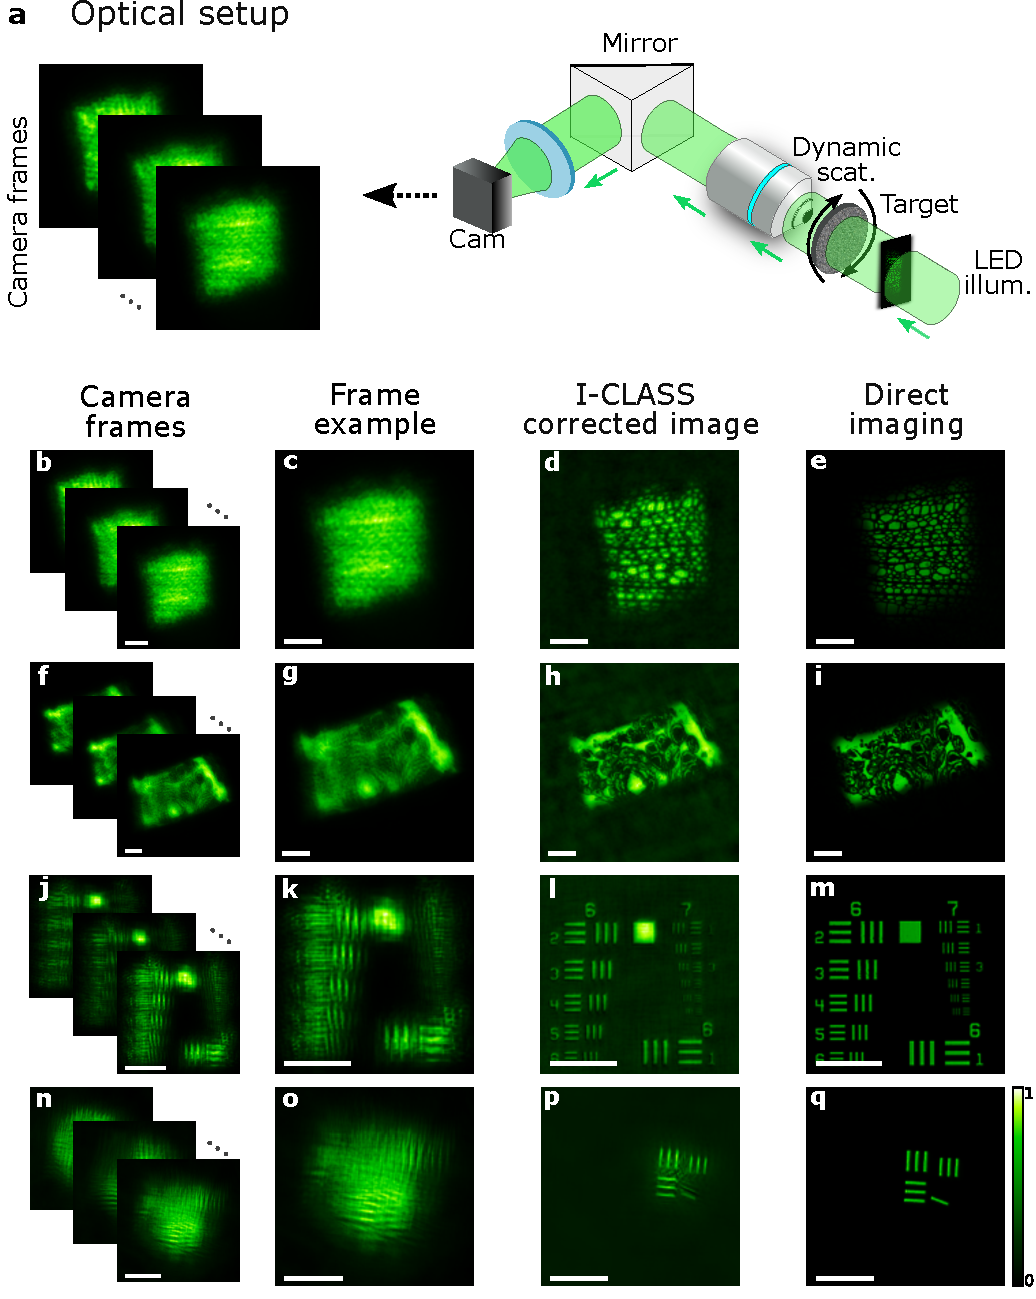
\includegraphics [width=0.96\textwidth,]
	{figures/figure_2.pdf}
    \caption{\textbf{Incoherent imaging proof of principle through a dynamic diffuser}.
   \textbf{a} Experimental setup: a conventional widefield microscope records $M=150$ distorted images of incoherently-illuminated targets through a dynamically rotating scattering diffuser. 
    \textbf{b,c} Captured raw camera frames.
    \textbf{d} I-CLASS corrected image, revealing the fine details and features of the target. The reconstructed PSF is given in Supplementary Section S1 and Supplementary Movie S1.
    \textbf{e} Reference image of the object as imaged without the diffuser present.
    \textbf{f-q} Same as b-e for different target objects and diffusers.
    %The rotating scattering diffuser was positioned 6mm from the targets for all measurements. The reconstruction of the time-varying PSFs using frame-wise deconvolution is given in Supplementary Section S1 and supplementary movies S1 and S2. 
    Colormaps are scaled between the minimum and maximum values of each reconstruction. Scale bars, 100 $\mu m$}
    \label{fig2}
\end{figure} 


Fig.~\ref{fig2}b-q presents the experimental imaging results after applying the I-CLASS reconstruction algorithm. 
Example raw captured frames of the target objects distorted by the diffuser are given in Fig.~\ref{fig2}b,c,f,g,j,k,n,o. As expected, the details of the objects are distorted due to scattering compared to their direct imaging without the diffuser present  (Fig.~\ref{fig2}e,i,m,q). The reconstructed images obtained by applying the I-CLASS algorithm \cite{weinberg2023noninvasive} on the captured frames (after multiplying each frame in Fig.~\ref{fig2}b,c,f,g by a fixed scalar value between 1 and 2, see Methods and Supplementary Section 2) reveal fine details and features of the objects, are presented in Fig.~\ref{fig2}c,g,k,o. %For comparison, Fig.~\ref{fig2}(E,I,M,Q) shows direct imaging of the objects without the scattering layers. 
%The rotating diffuser was positioned 6 mm from the targets for all measurements, with scale bars representing 100 $\mu m$. 
The reconstructed object allows estimation of the PSF of each frame by frame-wise deconvolution of each of the raw captured frames with the reconstructed object (Supplementary Section S1). Examples for the full dataset of captured frames, reconstructed objects, and reconstructed PSFs %of the experimental camera images, including the I-CLASS reconstructions of both the objects and the reconstructed PSFs for each frame, is 
are presented in Supplementary Section S1 and Supplementary Videos S1 and S2.

%The imaging process utilized an sCMOS camera (Neo 5.5, Andor), arranged in a 4f microscope setup with a $300mm$ tube lens and a 10x objective lens (MY10X-803, 0.28NA) for a total magnification $Mx \approx 15$, to capture the scattered image of the object effectively.

%%%%%%%%%%%%%%% Figure 3 - cuvette %%%%%%%%%%%%%%%%%%%%%%
\begin{figure}[b!]
	\centering
	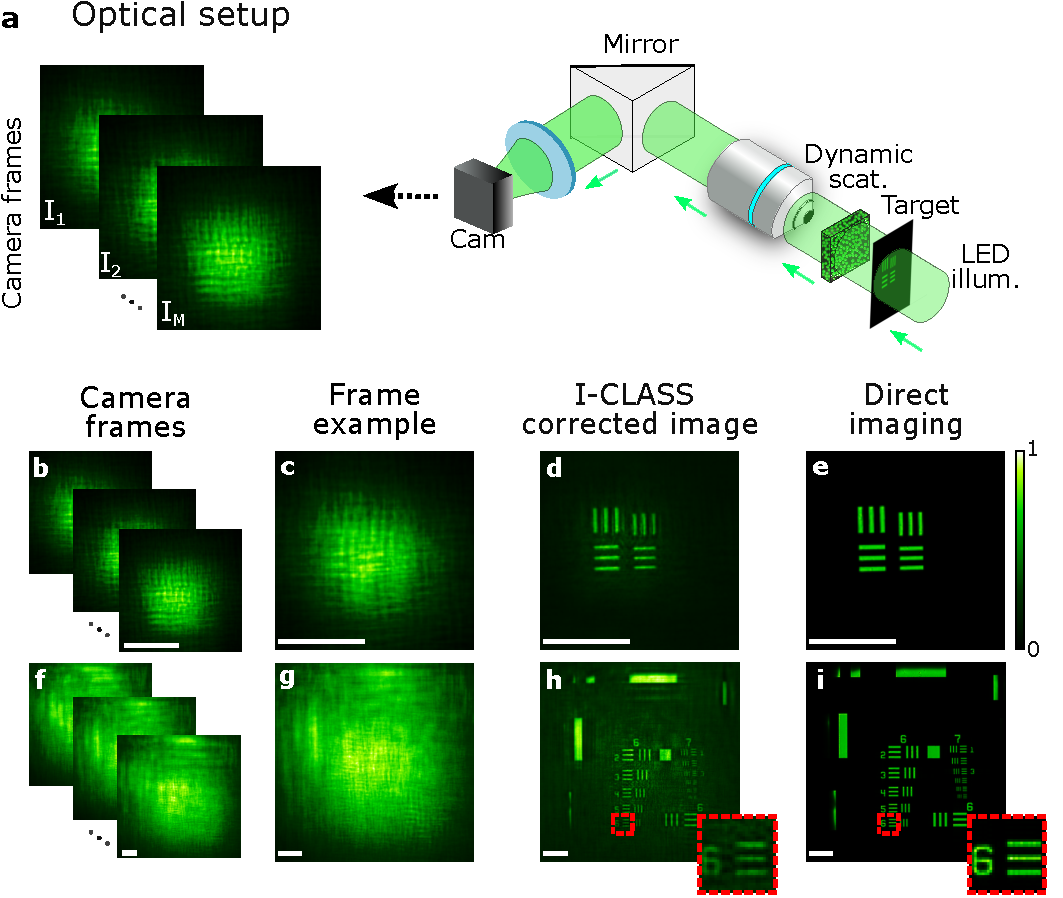
\includegraphics [width=0.99\textwidth,]
	{figures/figure_3.pdf}
    \caption{\textbf{Incoherent imaging through dynamic scattering}
    %\textbf{a} Setup: similar to Fig.~\ref{fig2}a, with a rotating diffuser replaced by a 1mm path length cuvette filled with 45 $\mu m$ polystyrene beads and a static holographic diffuser.
       \textbf{a} Experimental setup: a conventional widefield microscope records $M=150$ distorted images of incoherently-illuminated targets through a $1mm$-thick cuvette filled with a solution of 45 $\mu m$ polystyrene beads. A static diffuser is added in front of the cuvette to ensure no ballistic component is present. 
    \textbf{b,c} Experimental camera frames of target imaged through a dynamically rapidly varying medium taken at distinct times. \textbf{d}  I-CLASS reconstructed images. \textbf{e} Images of the object with the cuvette removed.
    \textbf{f-j} Same as b-e for different target objects.
    %The cuvette was positioned at 10mm (b) and 15mm (e) distances from the targets. 
    Insets in (h,i) show zoomed-in areas marked by red-dashed lines. Colormaps are scaled between the minimum and maximum values of each reconstruction. Scale bars, 150 $\mu m$}
    \label{fig3}
    \end{figure} 



As a second demonstration, we performed transmission imaging through a naturally-dynamic scatterer. To this end, we replaced the rotating diffuser with a $1mm$-thick cuvette containing 45$\mu m$-diameter Polystyrene beads in solution, creating a dynamically varying scattering as the beads flow freely in the suspension. Additionally, a static diffuser with a $0.5 ^\circ$ scattering angle was placed adjacent to the cuvette to ensure no ballistic component was present in the captured scattered light images. The experimental setup and results for these experiments are presented in Fig.~\ref{fig3}. 
Using this configuration, we imaged and reconstructed two resolution test targets. The captured camera frames (Fig.~\ref{fig3}b,f, and c,g) appear highly blurred, exhibiting no clear features. However, the I-CLASS corrected images (Fig.~\ref{fig3}d,h,l) successfully reconstruct the fine features of the target objects, demonstrating the effectiveness of the approach in correcting such natural dynamic scattering where no ballistic component is present. For reference, direct images of the same resolution targets captured without the scattering medium, using the same widefield transmission microscope, are provided in Fig.~\ref{fig3}e,i,m.

\textbf{Note:} The matrix-based imaging approach demonstrated here highlights the fundamental principle of imaging through dynamic scattering media. Although these initial experiments utilize a transmission geometry with illumination from behind the sample, our subsequent experimental demonstrations in fluorescence microscopy (Fig.~\ref{fig4}) and coherent holographic imaging (Fig.~\ref{fig5}) showcase the technique's adaptability across diverse optical configurations and imaging modalities.


% The targets
% were fabricated on 1.5mm thick glass slides coated with Ti and Ag. The Ti layer was 20nm thick
% placed above an Ag coating of 100nm thickness, fabricated using E-Beam Lithograph

% Measurements
% (B-E) 03-Mar-2024 [measurement 17, GT 14] (Icam[:,200:1000, 300:1100], gt[100:900, 150:950])
% (E-G) 03-Mar-2024 [measurement 10, GT 1] (Spatial Cut 100:1900,200:2000), gt[100:1900,200:2000] Fourier cut 500x500, post-process cut [100:450,50:400], inset cut[265:295,130:160]





\subsubsection*{Application to fluorescence microscopy}

As an additional proof of principle we tested our approach in a fluorescence microscopy experiment performed in epi-detection geometry through dynamic scattering. %with each rotation step ensuring an uncorrelated scattering pattern. 
The setup for this experiment is depicted in Fig.~\ref{fig4}a. It is a conventional widefield fluorescence microscope with a rotating diffuser placed between the microscope objective and the fluorescent sample (see Methods). The illumination source is a narrowband spatially-incoherent source composed of a 200-mW CW laser (06-MLD-488, Cobolt) and a rapidly rotating diffuser (see Methods). 
%The target objects were positioned behind a holographic diffuser mounted on a slowly rotating mount for $M$ discrete steps (K10CR1, Thorlabs ). This configuration was designed to produce uncorrelated point spread functions (PSFs) for each image acquisition. 
An sCMOS camera (Andor Neo 5.5) captures $M=150$ images of the scattered fluorescence light through a dichroic mirror and appropriate emission filters. %Exposure times were selected to ensure consistent illumination by averaging over sufficient illumination patterns. %. The system is arranged with a 300mm tube lens and a 10x objective lens (MY10X-803, 0.28NA) for a
%with a total magnification of $Mx \approx 15$, effectively capturing the scattered image of the object.

% Measurments
% (B-D) 16-Sep-2024 [measurement 6, GT 5] 
% (E-G) 16-Sep-2024 [measurement 3, GT 1] 

%%%%%%%%%%%%%% Figure 4 - FLUORESCENCE %%%%%%%%%%%%%%%%%%%%%%
\begin{figure}[htb!]
	\centering
	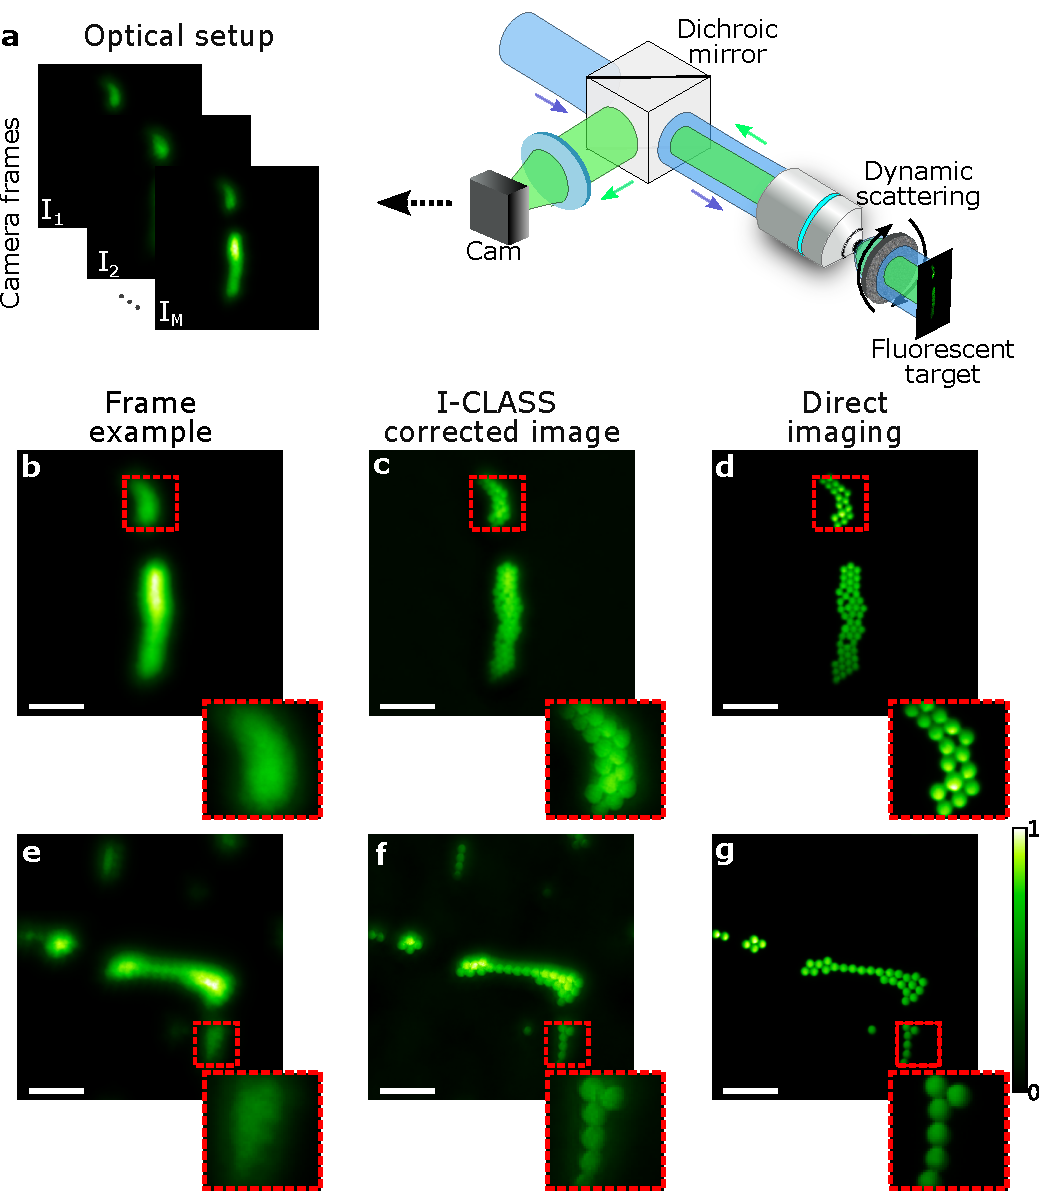
\includegraphics [width=1.03\textwidth,]
	{figures/figure_4.pdf}
    \caption{\textbf{Fluorescence microscopy through dynamic scattering}
    \textbf{a} Experimental setup: a conventional widefield fluorescence microscope records $M=150$ distorted images of fluorescent $10\mu m$-diameter beads through a dynamically rotating scattering diffuser.
    \textbf{b} Experimental camera frames of fluorescent objects imaged through an optical diffuser, showing distorted images due to scattering.
    \textbf{c} I-CLASS corrected images reveal fine details and features of the objects.
    \textbf{d} Reference images of the objects without scattering layers. \textbf{e-g} Same as b-d for different target objects. 
    Insets in b-g show zoomed-in areas marked by red-dashed lines. Colormaps are scaled between the minimum and maximum values of each reconstruction. Scale bars, 100 $\mu m$}
        \label{fig4}
    \end{figure} 


Fig.~\ref{fig4} presents the result of the fluorescence microscopy experiments. Fig.~\ref{fig4}b,e show sample captured frames of two targets composed of fluorescent beads (Fluoresbrite YG microspheres 10$\mu m$), as conventionally imaged through the optical diffuser. The significant distortion due to scattering can be observed in both the raw frames and the zoomed-in areas marked by red-dashed lines. The I-CLASS reconstructed images (Fig.\ref{fig4}c,f), after multiplying each frame by a fixed scalar value (see Methods and Supplementary Section 2), successfully recover fine details and features of the objects. For comparison, Fig.~\ref{fig4}d,g display the direct images of the objects as imaged without the scattering present.
%The rotating diffuser was positioned $\approx 8 mm$ from the targets for all presented camera frames, with scale bars representing $100 \mu m$.



%\subsection*{Experimental Results: Coherent Imaging}
%\subsubsection*{Holographic Coherence-gated Imaging}
%As a final demonstration of the approach's applicability to various experimental settings and imaging modalities, we apply it to a holographic dataset from coherent reflective measurements (Fig. XX). 

%Here, we demonstrate an experimental holographic measurement using holographic time-tagging of an object hidden behind a dynamically changing scattering sample, corrected with the same reconstruction method presented in the previous chapters. This approach is effective because focused illumination on the scattering sample, smaller than the correlation width of the scattering sample, induces a relatively stable illumination pattern, even for a dynamically changing scatterer. Fig. XX depicts the experimental setup used for this experiment: a target object is placed behind a scattering diffuser, and back-reflected scattered light fields are captured in a single-shot off-axis holography setup...

\pagebreak

\subsection*{Experimental results: holographic coherent imaging}

%\subsubsection*{Holographic coherent imaging}

As a final demonstration of the generality of the approach and its applicability to various imaging modalities, we applied it to coherent holographic reflective imaging. The results of this study are presented in Fig.~\ref{fig5}. 
The experimental setup is schematically depicted in Fig.~\ref{fig5}a: a reflective target (USAF resolution target) is illuminated by a wide illumination beam through a dynamically rotating diffuser. The illumination is provided by a $632$ nm Gaussian beam from a Helium-Neon laser (HNL210L, Thorlabs), which is focused to a tight spot on the diffuser surface to ensure that the object illumination remains relatively constant while the diffuser is varied (see below). 
An sCMOS camera holographically records $M=180$ reflected scattered light fields by imaging the diffuser back surface with a 4-f imaging system. A reference beam with a proper optical path delay matching the target distance is used for off-axis holographic acquisition \cite{cuche2000spatial}. %The reference arm is set to an optical path delay that matches the target distance, ensuring proper coherence-gating.

%The object, a USAF target, was placed approximately 7 cm behind the diffuser. A 4f imaging system with 1.6$\times$ magnification was used to image the diffuser onto the camera.
%In this experiment, we acquired $M=180$ holographic captures (Fig.~\ref{fig5}b), each using off-axis holography (see Fig.~\ref{fig5}a). 
To reconstruct the target, each captured field was digitally propagated to the target plane using Fresnel propagation (see Methods). As expected, without scattering compensation, the reconstructed fields are highly distorted, and the target object features cannot be observed (Fig.~\ref{fig5}b). %can be displayed a distorted version of the object amplitude (Fig.~\ref{fig5}c).\textbf{ }

% A critical challenge in the coherent configuration is ensuring that the illumination remains constant despite the rotation of the diffuser, which introduces dynamic scattering variations. This is done by focusing the illumination beam on the scattering facet, ensuring that the beam waist is smaller than the correlation length of the diffuser. As a result, the illumination pattern at the object's plane remains stable through the scan, providing consistent illumination.

If the image-forming equation has the same form as Eq.~\ref{eq:4}, the CTR-CLASS or I-CLASS algorithms can be directly applied to the holographically-captured fields. However, different from the spatially incoherent illumination case (Figs.2-4), where the illumination at the target plane was homogeneous regardless of the scattering layer dynamics, a significant challenge in the coherent imaging configuration is ensuring a constant illumination of the target despite the dynamic scattering introduced by the rotating diffuser. %In the spatially incoherent illumination case (Figs.2-4), the illumination at the target plane is rather spatially-homogeneous, either with or without the scattering diffuser present in the illumination path. 
Specifically, in the coherent illumination case (Fig.~\ref{fig5}), the presence of the dynamic scatterer in the illumination path of a wide beam generates a speckle illumination field at the target plane that may be subject to variations between scatterer realizations. Consequently, the measured field at the camera for the $m^{th}$ realization, $E^{cam}_m(\vec{r})$, can be expressed as:
\begin{equation}
E_m^{cam}(\vec{r})=P^{coh}_m(\vec{r}) * \left[ O(\vec{r}) E_m^{{ill}}(\vec{r}) \right]
\label{eq:5}
\end{equation}
Where $E_m^{{ill}}(\vec{r})$ is the illumination field at the target plane at the $m^{th}$ realization, $P^{coh}_m(\vec{r})$ denotes the complex-valued field amplitude point spread function (APSF) introduced by the scattering medium in the $m^{th}$ realization, and $O(\vec{r})$ is the target object spatial reflectivity. From Eq. \ref{eq:5} it is evident that if the illumination pattern remains unchanged across scattering realization: $E_m^{{ill}}(\vec{r})=E^{{ill}}(\vec{r})$, then \(O(\vec{r}) E^{{ill}}(\vec{r})=O^{{eff}}(\vec{r})  \), may be considered as an effective static object serving as the single object function that is assumed in the model of  From Eq. \ref{eq:4}.
To ensure this is the case, we have focused the Gaussian illumination beam on the scattering layer surface such that the beam waist at the scattering layer surface is sufficiently smaller than the correlation length of the scattering layer. This minimizes variations in $E_m^{{ill}}(\vec{r})$ between realizations, allowing the illumination field to be treated as effectively constant.
Under this assumption, the measured fields follow the equation:
\begin{equation}
E_m^{cam}(\vec{r}) \approx P^{coh}_m(\vec{r}) * O^{{eff}}(\vec{r})
\label{coherent eq.}
\end{equation}
Since Equations \ref{coherent eq.} and \ref{eq:4} share the same form, the CTR-CLASS \cite{lee22} can be applied to the measurements $E^{cam}_m(\vec{r})$, allowing the efficient reconstruction of the object field phase at the scattering layer plane. To reconstruct both the phase and amplitude of the object field, we applied the I-CLASS algorithm \cite{weinberg2023noninvasive}, which also estimates the object field amplitude from the $M$ captured fields. 
%The captured fields were reconstructed using the\textbf{I-CLASS} algorithm to compensate for scattering, 
The I-CLASS reconstructed object field at the scattering layer plane is numerically propagated to the target plane by Fresnel propagation (see Methods) to reconstruct the target, faithfully retrieving the fine features of the target (Fig.~\ref{fig5}d). 
With the reconstructed target obtained, the APSF for each frame, $P^{coh}_m(\vec{r})$, can be estimated. This can be achieved by calculating the phase introduced by the rotating diffuser at each realization, by taking \cite{sunray2024beyond}:
$\hat{P}^{coh}_{m}(r) = \mathcal{F} \left\{ e^{i \hat{\phi}_{diff}} \right\} = \mathcal{F} \left\{ e^{i \, \arg \left( \frac{E_m^{cam}(r_{cam})}{E_{CLASS}(r_{cam})} \right)} \right\}$
%$\hat{P}^{coh}_{m}(r)=\mathcal{F}\{ e^{i\hat{\phi}_{diff}} \}=\mathcal{F}\{e^{i\ arg ({E_m^{cam}(r_{cam})}/{E_{CLASS}(r_{cam})} )}\}$, where $E_m^{cam}$ 
are the measured fields at the diffuser plane, and $E_{CLASS}$ is the CLASS reconstructed object field at the diffuser plane. As shown in previous works \cite{choi2022flexible,sunray2024beyond}, the CLASS reconstructed object field also contains the spherical phase from the propagation distance between the object and the scattering layer. Thus, $\hat{\phi}_{diff}$ provides an estimation of the diffuser phase. 
Several estimated APSF are shown in Figure~\ref{fig5}e. 

%%%%%%%%%%%%%% Figure 5 - COHERENT %%%%%%%%%%%%%%%%%%%%%%
\begin{figure}[htb!]
	\centering
	\includegraphics [width=0.99\textwidth,]{figures/figure_5.pdf}
    \caption{\textbf{Experimental coherent reflection-imaging through dynamic scattering.} 
    \textbf{a} Experimental setup: A reflective target is illuminated through a dynamically rotating scattering diffuser. $M=180$ reflected light fields are holographically recorded in an off-axis holography configuration using a reference arm. %The illumination beam is focused to a tight spot on the diffuser surface such that the object illumination remains relatively constant while the diffuser is rotated.
    \textbf{b} Example of the recorded distorted fields after computational propagation to the object plane. \textbf{c} One example of the recorded field intensity after computational propagation to the object plane. 
    \textbf{d} Reconstructed object intensity at the object plane after applying the I-CLASS algorithm to compensate for scattering, revealing the details of the target. 
\textbf{e} Complex-valued field amplitude PSFs (APSFs), estimated from the captured fields after effective deconvolution of the reconstructed object field. 
\textbf{f} Reference intensity image of the object without the diffuser present. Scale bars, 1$mm$}
    \label{fig5}
\end{figure}

\section*{Discussion}
% Structure:
% - One can get the various PSFs using frame-wise deconvolution
% - Needs fixed illumination and static object requirement
% - unlike I-class single frame object estimation (and no averaging)
% - Isoplanatic correction

We have introduced and experimentally demonstrated a computational matricial framework for imaging through dynamic scattering media. The proposed framework addresses an important challenge in both coherent and incoherent imaging, which conventional matrix-based approaches have difficulty in tackling due to their reliance on multiple measurements within the scattering medium decorrelation time. 

Importantly, we have shown that under isoplanatic scattering conditions, the covariance matrix of dynamically scattered light fields has the same mathematical form as that of a conventional reflection matrix, with the roles of the medium and target object replaced. 
Thus, any matrix-based technique capable of decomposing the 'reflection-matrix' to an object field and scattering layer can be applied to reconstruct the hidden target. 
We chose to use the recently introduced I-CLASS algorithm due to the memory-efficient implementation developed in \cite{weinberg2023noninvasive,sunray2024beyond}, which allows high pixel-count processing and also the estimation of the object Fourier amplitude.

%A notable extension of the proposed framework is its ability to achieve different PSFs over time using frame-wise deconvolution with the retrieved static object (Supplementary Section S1).% Furthermore, this capability allows for adaptation to varying scattering conditions.

We note that while single-shot speckle-correlation approaches \cite{katz14} can, in principle, be applied to each of the captured frames since they only use the spatial autocorrelation of a single frame (or an estimation of a single autocorrelation from a set of frames as in stellar speckle interferometry \cite{labeyrie1970attainment}), their performance in terms of reconstruction fidelity for complicated objects and convergence stability are significantly inferior to the proposed covariance-matrix based approach (see numerical study in Supplementary Section S3).

%Unlike conventional speckle-correlation imaging techniques such as stellar speckle interferometry or single-shot autocorrelation-based imaging, which focus only on the diagonal of the covariance matrix, our approach utilizes the entire covariance matrix without any initial spatial averaging. This enables the reconstruction of highly complex scenes (Supplementary Section S3).

%Unlike CTR-CLASS \cite{lee22,sunray2024beyond} and I-CLASS \cite{weinberg2023noninvasive}, which fix each randomly illuminated frame distorted by the same scattering PSF and calculate the variance of the corrected images, our approach retrieves a single estimated image of the object that exhibits greater susceptibility to errors. %This limitation is directly attributable to the absence of multi-correction averaging, which underpins the disparities in performance and applicability between the two methods.

% KEEP FOR OURSELVES FOR NOW (Benzy - add to PhD proposal): While the proposed approach enables tackling rapidly varying scattering media, its main constraint is the assumption of a static target throughout the measurements. Nonetheless, the assumption of a static target in Eq.~\ref{eq:4} can still be maintained in scenarios where the target moves laterally throughout the measurements. Since, due to the convolution form of Eq.~\ref{eq:4}, a shift in the target object is mathematically equivalent to a shift of the PSF, which is naturally incorporated in the varying PSF model.
%varied effectively be seen as the movement of the PSF, not the scene itself, thanks to the shift ambiguity of the convolution operation. This adaptation broadens our method's applicability.

Finally, while we have focused our proof-of-principle demonstrations on isoplanatic scattering conditions, the field of view can be extended in anisoplanatic scattering conditions in cases of weakly scattering samples by individually reconstructing and mosaicking different isoplanatic patches \cite{trussell1978sectioned,alterman2021imaging,lee22,najar2024harnessing,sunray2024beyond}.
%another limitation of our method is the constrained field of view, determined by the optical memory effect or the 'isoplanatic' patch size \cite{katz14,osnabrugge2017generalized,weinberg2023noninvasive}. 
%In cases of weakly scattering samples, it may be possible to expand the corrected field of view by individually reconstructing and mosaicking different isoplanatic patches of the object, such as by cropping the image at the image plane \cite{trussell1978sectioned,alterman2021imaging,lee22,najar2024harnessing,sunray2024beyond}.



\section*{Materials and methods}

\subsection*{Experimental setup}

Figs.~\ref{fig2},\ref{fig3} show the experimental imaging configuration that utilizes an incoherent Thorlabs M625L3 LED light source. This LED emits at a central wavelength of $\lambda = 625$nm with an output power of 700mW and a full width at half maximum (FWHM) bandwidth of $\Delta \lambda = 17$nm. The emitted light covers an extensive area across the target plane located 3cm away. Image capture is conducted using an Andor Neo 5.5 sCMOS camera, part of a 4f imaging system equipped with a 10x Mitutoyo objective lens (M Plan APO 10X, NA 0.28) and a Thorlabs LA1256-A tube lens (focal length $300$mm). A Thorlabs FBH630-10 band-pass filter, with a central wavelength of $630$nm and a $10$nm FWHM, is employed to filter the incident light.

During the experiments in Fig.~\ref{fig2}, the dynamic media was created using a Thorlabs K10CR1 rotation mount with a holographic diffuser 6mm from the target. For Fig.~\ref{fig4}b-m, a Newport 0.5$^\circ$ holographic diffuser was used, and Fig.~\ref{fig2}n-q utilized an RPC Photonics EDC-1$^\circ$ diffuser.
For Fig.~\ref{fig3} experiments, scattering was introduced via a 1mm path-length cuvette containing Polystyrene beads (Fluoresbrite YG microspheres, 45 $\mu m$) in a solution with a concentration variability (c.v.) $\gg$ 7\%. A 0.5$^\circ$ holographic diffuser was attached to the cuvette to eliminate the scatterer's ballistic components. This scatterer was distanced $10mm$ for the measurements in Fig.~\ref{fig3}b-e and $15mm$ in Fig.~\ref{fig3}f-j.

The imaging targets varied across experiments. Figs.~\ref{fig2}b-e,\ref{fig2}f-i show prepared microscope slides by Maxlapter (Amazon) of willow stem and pine stem respectively. Figs.~\ref{fig2}j-m and \ref{fig3}f-j show a 3" x 3" Negative 1951 USAF Test Target (R3L3S1N, Thorlabs), and Figs.~\ref{fig2}n-q,\ref{fig3}b-e featured custom targets on 1.5mm thick glass slides coated with Ti (20nm) and Ag (100nm) layers, created through E-Beam Lithography.

Fig.~\ref{fig4} shows the fluorescence experimental configuration, which consists of a pseudothermal source composed of a 200-mW, 488nm continuous-wave (CW) laser (06-MLD-488, Cobolt) and a rapidly rotating holographic diffuser (EDC-1$^\circ$) at a distance of $\approx 15cm$ from the objective lens. The images were distorted by a discreetly rotating holographic diffuser (RD, NEWPORT 0.5$^\circ$) using a stepper motor rotation mount (K10CR2, Thorlabs) placed at distances of $\approx 8$mm from the target object. The images were captured using the same Andor Neo 5.5 sCMOS camera, imaged by a 4f imaging system equipped with a 10x Mitutoyo objective lens (M Plan APO 10X, NA 0.28) and a tube lens (focal length $300mm$, Thorlabs). The light was filtered with a dichroic mirror (DMLP505R, Thorlabs) and an emission filter (MF525-39, Thorlabs). The target consisted of fluorescent beads (Fluoresbrite YG microspheres 10$\mu m$) placed on a cover glass at the objective lens's focal plane.

Fig.~\ref{fig5} shows the experimental configuration for the coherent imaging experiments, where holograms were recorded using an off-axis holography setup. A 21-mW polarized CW He-Ne laser (HNL210L, Thorlabs) with a wavelength of 632.8 nm was used for illumination. To split the beam into reference and object paths, a polarizing beam splitter (PBS, PBSW-633, Thorlabs) was employed, with the path difference between the reference and object paths kept within the coherence length of the laser (~30 cm). After the PBS, the signal beam was rotated using a half-wave plate (WPQ10ME-633, Thorlabs) to match the polarization of the reference beam, allowing them to interfere at the detector. In the object path, the laser beam passed through a Newport 0.5$^\circ$ holographic diffuser mounted on a rotating motor (K10CR1, Thorlabs), ensuring uncorrelated scattering patterns due to the diffuser's rotation. A 10X Mitutoyo objective lens (M Plan APO 10X, NA 0.28) focused the illumination beam, ensuring the illumination spot on the diffuser was smaller than the diffuser's correlation length (~70 $\mu$m), maintaining consistent illumination. The negative USAF test target (R1DS1N, Thorlabs) was positioned approximately 7 cm behind the diffuser, with a mirror covered by a diffusive slide placed behind it to simulate a diffusive object. The reflected light traveled back through the diffuser to the camera. A 4f imaging system consisting of two lenses, an $f=200$ mm (AC508-200-A-ML, Thorlabs) and an $f=125$ mm (LA1384-A, Thorlabs), was used to image the field at the diffuser plane onto the camera sensor (Thorlabs 8051M-USB), providing a magnification of 1.6$\times$. A non-polarizing beam splitter (BS03, Thorlabs) was used to recombine the object and reference beams before interfering at the camera plane. Finally, a band-pass filter (MaxLine Laser Line Filter 633) with a center wavelength of 632.8 nm and a bandwidth of 1 nm was positioned in front of the camera to isolate the laser wavelength and reduce noise.



\subsection*{Experimental Parameters}

The experimental parameters for the results displayed in Figs.~\ref{fig2}, \ref{fig3}, \ref{fig4}, and \ref{fig5}, including camera exposure times and image pixel counts, are outlined as follows:

The frames in Fig.~\ref{fig2}b-e were captured at 1250×1250 pixels, each taken at a 0.9 ms exposure time. In Fig.~\ref{fig2}f-i, images were captured at a resolution of 1700×1700 pixels and then cropped in the Fourier domain to 300×300 pixels, with an exposure time of 0.5 ms. In Fig.~\ref{fig2}j-m, frames were captured at 700×700 pixels with a 1.25 ms exposure time. Fig.~\ref{fig2}n-q features frames captured at 800×800 pixels, cropped in the Fourier domain to 300×300 pixels, with an exposure time of 7 ms.
For Figs.\ref{fig3}b-e, frames were sized at 800×800 pixels, each with a 50 ms exposure time. In Fig.~\ref{fig3}f-i, images were captured at a resolution of 1800×1800 pixels, first cropped in the Fourier domain to 300×300 pixels and then further cropped to 350×350 pixels for visualization, with an exposure time of 30 ms per frame.
In Fig.~\ref{fig4}b-e, frames were captured at 750×750 pixels and cropped in the Fourier domain to 500×500 pixels, with an exposure time of 0.275 s per frame. Similarly, in Fig.~\ref{fig4}f-j, frames were captured at 650×650 pixels, cropped in the Fourier domain to 300×300 pixels, with an exposure time of 0.25 s
In Fig.~\ref{fig5}, the object frames were initially captured at 850×850 pixels and cropped to 350×350 pixels for visualization, with an exposure time of 12 ms per frame.
Experiments shown in Figs.~\ref{fig2}b-m,\ref{fig3},\ref{fig4} utilized $M=150$ realizations for reconstruction, while results in Figs.~\ref{fig2}n-q 
and \ref{fig5} used $M=180$.

We applied intensity modulation by multiplying each camera frame with a fixed scalar factor, linearly varying from 1 to 2 across frames 1-150, to suppress energy conservation-induced correlations in the PSFs for the measurements shown in Fig.~\ref{fig2}b-m and \ref{fig4}. This is discussed in more detail in Supplementary Section S2.

The algorithm run time on a commercially available GPU (Nvidia RTX4090, 24 GB) was approximately $\sim 200ms$ per iteration for 150 camera frames at a resolution of $1400 \times 1400$ pixels and around $\sim 50ms$ per iteration for 150 camera frames at a resolution of $700 \times 700$ pixels.


\subsection*{I-CLASS}
The full description of the I-CLASS memory-efficient, phase, and amplitude scattering compensation algorithm is fully given in Supplementary Section S4. Here, we provide a concise explanation of the I-CLASS algorithm.

\subsubsection*{Memory-efficient CLASS iterations}

The memory-efficient equivalent method for calculating the CLASS iterations using the $N \times M$ matrix $\hat{\textbf{A}}$ without the explicit computation of the $N \times N$ matrix $\textbf{R}_{virt}$ can be calculated from the following formula for the t-th iteration (see Supplementary S1): 

\begin{eqnarray}
\vec{z}_{t+1}=\sum_{q=1}^{M}(\tilde{\textbf{A}}_t^* \odot ((\tilde{\textbf{A}}_t^{(ud)^*}*\tilde{\textbf{A}}_t^{(lr)})_{:,M-1} \star \tilde{\textbf{A}}_t^{(ud)}))_{:,q}
\label{eq:three}
\end{eqnarray}

\noindent where $\tilde{\textbf{A}}$ as the 2D Fourier transform of $\hat{\textbf{A}}$. Here, $\tilde{\textbf{A}}^{(ud)}$ is the matrix $\tilde{\textbf{A}}$ with each of its columns flipped upside-down, and $\tilde{\textbf{A}}^{(lr)}$ is $\tilde{\textbf{A}}$ with its rows flipped left-to-right. In addition, we denote the element-wise Hadamard product as $\odot$, the 2D convolution as $*$, and the 2D correlation operator as $\star$. $\textbf{X}^{*}$ is the element-wise complex-conjugation operator on the matrix $\textbf{X}$, and $\textbf{X}_{:,q}$ is the q-th column of $\textbf{X}$.

As in the conventional CLASS algorithm \cite{kang17}, throughout the iterative process of the I-CLASS algorithm, we solely update the $\vec{k}$-space (OTF) phase correction with the correction:
\begin{eqnarray}
\tilde{\textbf{A}}_{t+1}=diag\{e^{i\frac{\vec{z}_t}{|\vec{z}_t|}}\}\tilde{\textbf{A}}_t
\end{eqnarray}
\noindent where the exponential and division operations are element-wise and $t=1...T$ is the iteration number. 
 \subsubsection*{I-CLASS $\vec{k}$-space amplitude correction}

The $\vec{k}$-space amplitude correction in the I-CLASS algorithm consists of two primary steps: (1) estimating the MTF, up to a scaling factor, using $\widehat{MTF} \equiv  \sqrt{diag\{ \tilde{\textbf{R}_{virt}} \}} = \sqrt{\sum_{q=1}^{M} (\tilde{\textbf{A}} \odot \tilde{\textbf{A}}^*)_{:,q}}$ (See supplementary S1). We note that this scaling factor ambiguity inhibits quantitative reconstruction unless the scattering medium transmission is properly estimated. (2) The estimated MTF is then utilized in a regularized Fourier reweighting on each of the captured camera frames after the phase-correction:%last iteration CLASS corrected object $\vec{{O}}_{CLASS}$:

\begin{eqnarray}
\tilde{\textbf{A}}_{fixed}=\frac{\tilde{\textbf{A}}_T}{\widehat{MTF}+\sigma}
\end{eqnarray}

%  \begin{eqnarray}
%      \vec{\tilde{O}}_{I-CLASS_{i}} \equiv \frac{ \vec{\tilde{O}}_{CLASS_{i}}}{\frac{\widehat{MTF}_i}{\max_{q} \widehat{MTF}_q }+\sigma}
% \end{eqnarray}

\noindent where $\sigma$ is the regularization parameter, and $\tilde{\textbf{A}}_T$ are the phase-corrected frames.  

As a final step, The phase and Fourier-amplitude corrected frames are then reconstructed by inverse Fourier transforming back the corrected Fourier matrix $\tilde{\textbf{A}}_{fixed}$ into $\hat{\textbf{A}}$ and taking the pixel-wise square root of the sum of the columns of $|\hat{\textbf{A}}|^2$ which is equivalent to the square root of the variance image, i.e. the square-root of the scattering-corrected virtual-confocal image (see supplementary S1). This can be written mathematically as $diag\{ \textbf{R}_{virt} \} = \sum_{q=1}^{M} (\hat{\textbf{A}} \odot \hat{\textbf{A}}^*)_{:,q}$, and the I-CLASS corrected object 
is given by taking an element-wise square root as seen from Eq.~\ref{eq:two}. We note that the I-CLASS final image inherently contains shift ambiguity, where a shift in the PSF can be equally interpreted as a shift in the target object. For convenience, in all the presented reconstructions, the images were co-registered with respect to the widefield reference.


\subsection*{Fresnel Propagation via Fourier-Domain Transfer Function}
\label{Fresnel_propagation}
In Fig.~\ref{fig5}, we present the object field located at the physical object plane, $z_{\text{obj}}$. However, the I-CLASS algorithm reconstructs the complex field in the plane of the scattering layer, denoted as $E_o(x, y, z_{\text{scatt}})$. To visualize the field at the object plane, we propagate the reconstructed field from the diffuser plane to the object plane using Fresnel propagation under the paraxial approximation.

This propagation is efficiently implemented in the Fourier domain using the Fresnel transfer function:

\begin{equation}
    E_o(x, y, z_{\text{obj}}) = \mathcal{F}^{-1} \left\{ \tilde{E}_o(f_x, f_y, z_{\text{scatt}}) \cdot H(f_x, f_y; \Delta z) \right\}
\end{equation}

where:
- $ \tilde{E}_o(f_x, f_y, z_{\text{scatt}}) = \mathcal{F}\{ E_o(x, y, z_{\text{scatt}}) \} $ is the 2D Fourier transform of the reconstructed field,
- $ H(f_x, f_y; \Delta z) $ is the Fresnel transfer function,
- $ \Delta z = z_{\text{obj}} - z_{\text{scatt}} $ is the propagation distance,
- $ \mathcal{F} $ and $ \mathcal{F}^{-1} $ denote the 2D Fourier and inverse Fourier transforms.

The Fresnel transfer function in terms of spatial frequency is:

\begin{equation}
    H(f_x, f_y; \Delta z) = \exp\left[ i \frac{2\pi \Delta z}{\lambda} \right] \cdot \exp\left[ -i \pi \lambda \Delta z (f_x^2 + f_y^2) \right]
\end{equation}

Here:
- $ \lambda $ is the illumination wavelength,
- $ (f_x, f_y) $ are the spatial frequency coordinates corresponding to the real-space axes $ (x, y) $.

This formulation supports forward and backward propagation by simply changing the sign of $ \Delta z $, and is especially suitable for numerical implementation via Fast Fourier Transforms.

\newpage


\subsection*{Funding}
\noindent This project was supported by the H2020 European Research Council (101002406).
\subsection*{Competing interests}
\noindent The authors declare no competing interests.
\subsection*{Author contributions}
O.K. proposed and conceptualized the project with E.S. and G.W.; E.S., G.W., and O.K. designed the incoherent imaging experimental setup. B.L. and O.K. designed the coherent imaging experimental setup. G.W. carried out the incoherent imaging measurements and data analysis with input from E.S.; B.L. carried out the coherent imaging measurements and data analysis. E.S. wrote the reconstruction algorithm code and numerical simulations with input from G.W.; O.K. supervised the project. All authors contributed to the writing of the manuscript.

\subsection*{Code availability}
For applying the I-CLASS algorithm, we used the published memory-efficient implementation described in \cite{weinberg2023noninvasive,sunray2024beyond}, using the code released with the paper. The code is publicly available at https://doi.org/10.5281/zenodo.11266090, and the up-to-date version can be found at https://github.com/Imaging-Lab-HUJI/Fluorescence-Computational-Imaging-Through-Scattering-Layers.

\subsection*{Data availability}
All data needed to evaluate the conclusions in the paper are present in the paper and/or the supplementary materials. Additional data related to this paper may be requested from the authors.

\bibliography{bib}

\end{document}
